% TODO checklist - Files inspected for this section:
% - README.md (lines 1-2050): Architecture overview, three-layer design, design rationale
% - Q&A.md (lines 1-7907): Q8-15 (architecture deep-dive), Q45 (maintainability/extensibility), Q46 (technical debt)
% - src/app.py: Application factory, middleware composition
% - src/middleware/: Cross-cutting concerns implementation
% - src/adapters/: Adapter pattern implementations
% - src/services/: Service layer design
% - docs/adr/: Architecture Decision Records (if available)
% - SECURITY.md: Defense-in-depth principles

\section{Design Principles}
\label{sec:design-principles}

This section articulates the design principles that guided architectural decisions for the Cineca Agentic Platform. These principles represent deliberate trade-offs optimized for enterprise deployment, operational excellence, and long-term maintainability.

%------------------------------------------------------------------------------
\subsection{Separation of Concerns: Three-Layer Architecture}
\label{subsec:three-layer}

The platform adopts a three-layer architecture that enforces clear boundaries between concerns:

\begin{figure}[htbp]
\centering
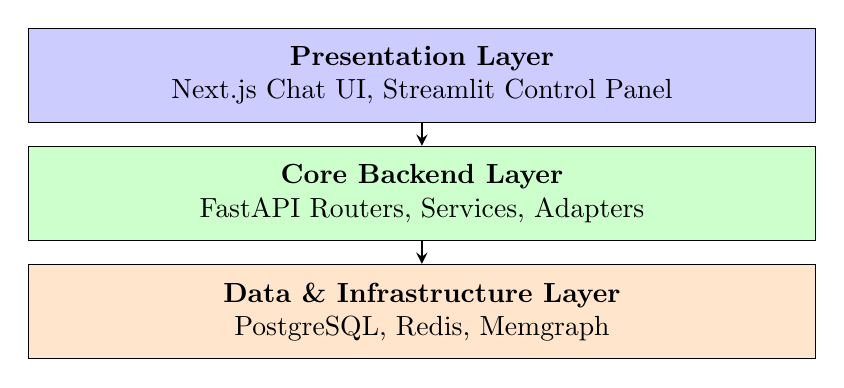
\begin{tikzpicture}[
    layer/.style={rectangle, draw, minimum width=10cm, minimum height=1.2cm, align=center},
    arrow/.style={->, thick, >=stealth}
]
    % Layers
    \node[layer, fill=blue!20] (presentation) at (0, 3) {\textbf{Presentation Layer}\\Next.js Chat UI, Streamlit Control Panel};
    \node[layer, fill=green!20] (core) at (0, 1.5) {\textbf{Core Backend Layer}\\FastAPI Routers, Services, Adapters};
    \node[layer, fill=orange!20] (data) at (0, 0) {\textbf{Data \& Infrastructure Layer}\\PostgreSQL, Redis, Memgraph};
    
    % Arrows
    \draw[arrow] (presentation.south) -- (core.north);
    \draw[arrow] (core.south) -- (data.north);
\end{tikzpicture}
\caption{Three-Layer Architecture}
\label{fig:three-layer}
\end{figure}

\subsubsection{Layer Responsibilities}

\begin{description}
    \item[Presentation Layer:] Responsible for user interaction, request formatting, and response rendering. The layer is stateless and communicates exclusively through the backend API. Technology choices (Next.js, Streamlit) can evolve independently of backend logic.
    
    \item[Core Backend Layer:] Contains business logic, orchestration, and API contracts. This layer is further subdivided into:
    \begin{itemize}
        \item \textbf{Router Layer:} HTTP endpoint handlers, request validation, response serialization
        \item \textbf{Service Layer:} Business logic, orchestration, transaction management
        \item \textbf{Adapter Layer:} External system integration (LLM providers, databases)
    \end{itemize}
    
    \item[Data \& Infrastructure Layer:] Provides persistent storage, caching, and external service integrations. This layer abstracts infrastructure details behind repository and adapter interfaces.
\end{description}

\subsubsection{Layer Coupling Rules}

\begin{itemize}
    \item Upper layers may depend on lower layers, but not vice versa
    \item The core backend layer defines interfaces that adapters implement
    \item Cross-layer communication occurs through well-defined contracts (Pydantic schemas, repository interfaces)
    \item Infrastructure concerns (connection pooling, retry logic) are encapsulated within the adapter layer
\end{itemize}

%------------------------------------------------------------------------------
\subsection{Defense in Depth: Security Layering}
\label{subsec:defense-in-depth}

Security is implemented through multiple overlapping defensive layers, ensuring that compromise of any single layer does not result in complete system breach:

\begin{table}[htbp]
\centering
\caption{Defense-in-Depth Security Layers}
\label{tab:security-layers}
\small
\begin{tabular}{|c|l|p{7cm}|}
\hline
\textbf{Layer} & \textbf{Name} & \textbf{Controls} \\
\hline
1 & Network & TLS encryption, firewall rules, network segmentation \\
\hline
2 & Authentication & OIDC/JWT validation, token expiration, JWKS verification \\
\hline
3 & Authorization & Scope-based RBAC, endpoint-level permission checks \\
\hline
4 & Tenant Isolation & Request-scoped tenant context, query-level filtering \\
\hline
5 & Input Validation & Pydantic schema validation, Cypher injection prevention \\
\hline
6 & Rate Limiting & Per-user/tenant quotas, sliding window throttling \\
\hline
7 & Output Filtering & PII scrubbing, response sanitization \\
\hline
8 & Audit & Append-only audit logs, tamper detection \\
\hline
\end{tabular}
\end{table}

\subsubsection{Security Principle Applications}

\begin{description}
    \item[Principle of Least Privilege:] Tokens carry minimal scopes required for the task. Administrative operations require explicit \texttt{admin:all} scope. Tool invocations check capability requirements before execution.
    
    \item[Fail Secure:] When authentication or authorization cannot be verified (e.g., JWKS unavailable), requests are denied rather than allowed.
    
    \item[Separation of Duties:] Administrative functions (tenant management, model configuration) are separated from operational functions (agent execution, job processing).
    
    \item[Defense Diversity:] Multiple security mechanisms (authentication, authorization, validation) use different implementation approaches to prevent single-point vulnerabilities.
\end{description}

%------------------------------------------------------------------------------
\subsection{Fail-Safe Defaults}
\label{subsec:fail-safe}

The platform implements fail-safe defaults that favor security and stability over permissiveness:

\begin{itemize}
    \item \textbf{Authentication Required:} All endpoints except health probes require valid JWT tokens. Unauthenticated requests receive 401 responses.
    
    \item \textbf{Restrictive RBAC:} New users receive minimal scopes (\texttt{user:me}). Elevated permissions must be explicitly granted.
    
    \item \textbf{Read-Only by Default:} Graph queries default to read-only mode. Write operations require explicit flags and \texttt{graph:write} scope.
    
    \item \textbf{Conservative Timeouts:} Default timeouts are set to prevent resource exhaustion (30 seconds for tools, 120 seconds for agent runs).
    
    \item \textbf{Rate Limiting Enabled:} Rate limits apply by default; exemptions require explicit configuration.
    
    \item \textbf{Audit Logging Enabled:} Security-relevant events are logged by default; suppression requires explicit opt-out.
    
    \item \textbf{Circuit Breakers Closed:} External provider circuits start closed; failures trigger protection automatically.
\end{itemize}

%------------------------------------------------------------------------------
\subsection{Extensibility and Modularity}
\label{subsec:extensibility}

The architecture prioritizes extensibility to accommodate future requirements without architectural rewrites:

\subsubsection{Extension Points}

\begin{table}[htbp]
\centering
\caption{Platform Extension Points}
\label{tab:extension-points}
\small
\begin{tabularx}{\textwidth}{|>{\raggedright\arraybackslash}p{2.8cm}|>{\raggedright\arraybackslash}X|>{\raggedright\arraybackslash}p{2.5cm}|}
\hline
\textbf{Extension Type} & \textbf{Mechanism} & \textbf{Effort Level} \\
\hline
New MCP Tool & Module creation at \texttt{src/mcp/tools/<category>/<name>.py} & Low (1 file, auto-discovered) \\
\hline
New LLM Provider & Adapter implementation in \texttt{src/adapters/llm.py} & Medium (1-2 files) \\
\hline
New API Endpoint & Router module in \texttt{src/routers/}, mount in \texttt{app.py} & Low (2-3 files) \\
\hline
New Background Task & Job type in \texttt{src/jobs/}, worker handler & Medium (2-3 files) \\
\hline
New Health Probe & Component in \texttt{src/health/components.py} & Low (1 function) \\
\hline
New Graph Domain & Schema in \texttt{db/memgraph\_domain/}, ETL loaders & Medium (3-5 files) \\
\hline
New Metric & Registration in \texttt{src/observability/metrics.py} & Low (1 declaration) \\
\hline
\end{tabularx}
\end{table}

\subsubsection{Modularity Principles}

\begin{description}
    \item[Single Responsibility:] Each module addresses one cohesive concern. Routers handle HTTP, services handle logic, adapters handle integration.
    
    \item[Interface Segregation:] Narrow interfaces prevent unnecessary coupling. The \texttt{JobStore} interface exposes only CRUD operations, not implementation details.
    
    \item[Dependency Inversion:] High-level modules (services) depend on abstractions (interfaces), not concrete implementations (Redis, PostgreSQL).
    
    \item[Convention over Configuration:] Tools are discovered by naming convention (\texttt{<category>.<name>} maps to \texttt{src/mcp/tools/<category>/<name>.py}), reducing boilerplate.
\end{description}

%------------------------------------------------------------------------------
\subsection{Observability by Design}
\label{subsec:observability-by-design}

Observability is not an afterthought but a core architectural concern integrated throughout the system:

\subsubsection{Instrumentation Principles}

\begin{itemize}
    \item \textbf{Request Correlation:} Every request receives a unique \texttt{request\_id} that propagates through logs, metrics, and traces for end-to-end visibility.
    
    \item \textbf{Structured Logging:} All log statements use structured format (JSON in production) with consistent field naming for log aggregation and querying.
    
    \item \textbf{Metric Granularity:} Metrics are labeled by relevant dimensions (endpoint, status, tenant) to support flexible aggregation and alerting.
    
    \item \textbf{Trace Sampling:} Distributed traces use configurable sampling (100\% in development, 20\% in production) to balance observability with overhead.
    
    \item \textbf{Health Semantics:} Health probes distinguish between liveness (process alive), readiness (accepting traffic), and component health (dependency status).
\end{itemize}

\subsubsection{Observability Integration Points}

\begin{figure}[htbp]
\centering
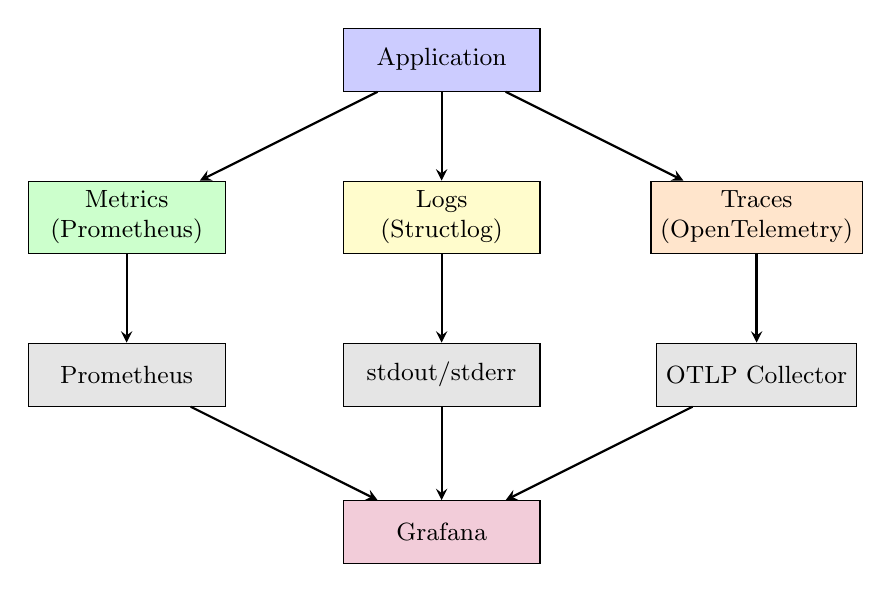
\begin{tikzpicture}[
    box/.style={rectangle, draw, minimum width=2.5cm, minimum height=0.8cm, align=center, font=\small},
    arrow/.style={->, thick, >=stealth}
]
    % Application
    \node[box, fill=blue!20] (app) at (0, 2) {Application};
    
    % Three pillars
    \node[box, fill=green!20] (metrics) at (-4, 0) {Metrics\\(Prometheus)};
    \node[box, fill=yellow!20] (logs) at (0, 0) {Logs\\(Structlog)};
    \node[box, fill=orange!20] (traces) at (4, 0) {Traces\\(OpenTelemetry)};
    
    % Backends
    \node[box, fill=gray!20] (prom) at (-4, -2) {Prometheus};
    \node[box, fill=gray!20] (stdout) at (0, -2) {stdout/stderr};
    \node[box, fill=gray!20] (otel) at (4, -2) {OTLP Collector};
    
    % Visualization
    \node[box, fill=purple!20] (grafana) at (0, -4) {Grafana};
    
    % Arrows
    \draw[arrow] (app) -- (metrics);
    \draw[arrow] (app) -- (logs);
    \draw[arrow] (app) -- (traces);
    \draw[arrow] (metrics) -- (prom);
    \draw[arrow] (logs) -- (stdout);
    \draw[arrow] (traces) -- (otel);
    \draw[arrow] (prom) -- (grafana);
    \draw[arrow] (stdout) -- (grafana);
    \draw[arrow] (otel) -- (grafana);
\end{tikzpicture}
\caption{Observability Data Flow}
\label{fig:observability-flow}
\end{figure}

%------------------------------------------------------------------------------
\subsection{Enterprise-First Design Trade-offs}
\label{subsec:enterprise-tradeoffs}

The platform makes deliberate trade-offs favoring enterprise requirements over prototyping simplicity:

\begin{table}[htbp]
\centering
\caption{Enterprise vs. Prototyping Trade-offs}
\label{tab:enterprise-tradeoffs}
\small
\begin{tabularx}{\textwidth}{|l|X|X|}
\hline
\textbf{Concern} & \textbf{Enterprise Choice} & \textbf{Alternative (Not Chosen)} \\
\hline
Authentication & Full OIDC with JWKS validation & Simple API key authentication \\
\hline
Authorization & Scope-based RBAC with audit & All-or-nothing access \\
\hline
Multi-tenancy & First-class tenant isolation & Single-tenant with instance-per-customer \\
\hline
Configuration & Database-backed with hierarchy & Environment variables only \\
\hline
Job Processing & PostgreSQL-backed with SSE & In-memory queues \\
\hline
Health Checks & Component-level with degradation & Simple ``up/down'' check \\
\hline
Metrics & 50+ Prometheus metrics & Basic request counters \\
\hline
Logging & Structured JSON with correlation & Plain text logs \\
\hline
API Versioning & Explicit /v1/, /v2/ paths & Unversioned endpoints \\
\hline
Error Responses & RFC 7807 Problem Details & Ad-hoc error formats \\
\hline
\end{tabularx}
\end{table}

\subsubsection{Trade-off Implications}

These enterprise-first choices have implications:

\begin{description}
    \item[Increased Complexity:] The codebase is larger and requires more infrastructure (Redis, PostgreSQL, OIDC provider) compared to minimal prototypes.
    
    \item[Steeper Learning Curve:] New developers must understand authentication flows, tenant context, and observability patterns.
    
    \item[Higher Operational Overhead:] Production deployment requires monitoring, alerting, and infrastructure management expertise.
    
    \item[Longer Initial Setup:] Development environment setup requires Docker Compose with multiple services versus a single Python process.
\end{description}

These implications are acceptable for the target enterprise context, where operational stability, security compliance, and maintainability outweigh initial simplicity.

%------------------------------------------------------------------------------
\subsection{Stateless API Design}
\label{subsec:stateless-api}

The API layer follows stateless design principles to enable horizontal scaling:

\begin{itemize}
    \item \textbf{No Server-Side Sessions:} Authentication state is carried in JWT tokens, not server-side session stores.
    
    \item \textbf{Externalized State:} All persistent state resides in PostgreSQL (authoritative) or Redis (ephemeral/cache).
    
    \item \textbf{Idempotent Operations:} Write operations support idempotency keys, enabling safe retry without side effects.
    
    \item \textbf{Cursor-Based Pagination:} Collection endpoints use stateless cursor tokens rather than offset-based pagination.
    
    \item \textbf{Request-Scoped Context:} Tenant context, request ID, and trace context are established per-request and do not depend on prior requests.
\end{itemize}

\subsubsection{Statelessness Benefits}

\begin{enumerate}
    \item \textbf{Horizontal Scaling:} Any API instance can handle any request; load balancers can route freely.
    
    \item \textbf{Failure Isolation:} Instance failure does not lose session state; clients can retry to any available instance.
    
    \item \textbf{Deployment Simplicity:} Rolling deployments do not require session draining or sticky sessions.
    
    \item \textbf{Testing:} Each request can be tested in isolation without setup/teardown of session state.
\end{enumerate}

%------------------------------------------------------------------------------
\subsection{Adapter Pattern for External Integration}
\label{subsec:adapter-pattern}

External systems (LLM providers, databases) are accessed through adapter interfaces that isolate integration complexity:

\begin{figure}[htbp]
\centering
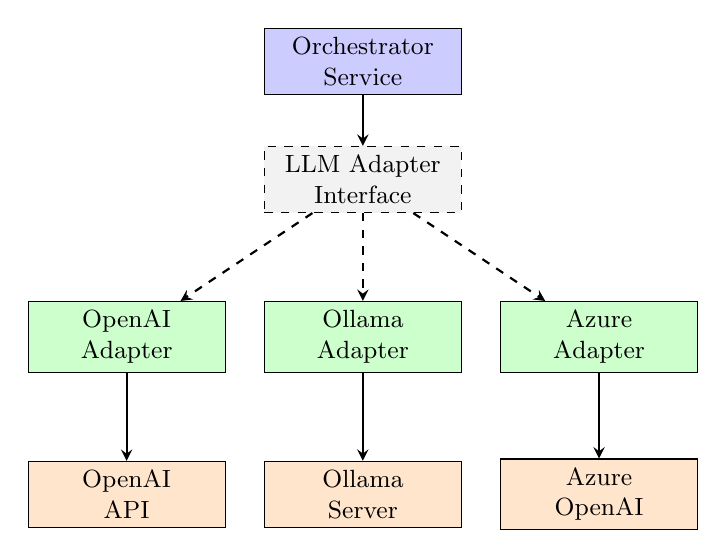
\begin{tikzpicture}[
    box/.style={rectangle, draw, minimum width=2.5cm, minimum height=0.8cm, align=center, font=\small},
    interface/.style={rectangle, draw, dashed, minimum width=2.5cm, minimum height=0.8cm, align=center, font=\small},
    arrow/.style={->, thick, >=stealth}
]
    % Service
    \node[box, fill=blue!20] (service) at (0, 2) {Orchestrator\\Service};
    
    % Interface
    \node[interface, fill=gray!10] (interface) at (0, 0.5) {LLM Adapter\\Interface};
    
    % Implementations
    \node[box, fill=green!20] (openai) at (-3, -1.5) {OpenAI\\Adapter};
    \node[box, fill=green!20] (ollama) at (0, -1.5) {Ollama\\Adapter};
    \node[box, fill=green!20] (azure) at (3, -1.5) {Azure\\Adapter};
    
    % External
    \node[box, fill=orange!20] (ext1) at (-3, -3.5) {OpenAI\\API};
    \node[box, fill=orange!20] (ext2) at (0, -3.5) {Ollama\\Server};
    \node[box, fill=orange!20] (ext3) at (3, -3.5) {Azure\\OpenAI};
    
    % Arrows
    \draw[arrow] (service) -- (interface);
    \draw[arrow, dashed] (interface) -- (openai);
    \draw[arrow, dashed] (interface) -- (ollama);
    \draw[arrow, dashed] (interface) -- (azure);
    \draw[arrow] (openai) -- (ext1);
    \draw[arrow] (ollama) -- (ext2);
    \draw[arrow] (azure) -- (ext3);
\end{tikzpicture}
\caption{Adapter Pattern for LLM Providers}
\label{fig:adapter-pattern}
\end{figure}

\subsubsection{Adapter Responsibilities}

Each adapter encapsulates:
\begin{itemize}
    \item Protocol translation (REST, gRPC, native client)
    \item Authentication with the external service
    \item Request/response mapping to internal schemas
    \item Error handling and retry logic
    \item Circuit breaker integration
    \item Metrics collection for the external call
\end{itemize}

%------------------------------------------------------------------------------
\subsection{Repository Pattern for Data Access}
\label{subsec:repository-pattern}

Data access follows the repository pattern, abstracting storage mechanics from business logic:

\begin{description}
    \item[Repository Interface:] Defines operations (create, read, update, delete, query) without exposing SQL or ORM details.
    
    \item[Tenant Scoping:] Repositories automatically scope queries by tenant ID, preventing accidental cross-tenant access.
    
    \item[Transaction Boundary:] Services control transaction boundaries; repositories operate within the provided session.
    
    \item[Query Optimization:] Complex queries are encapsulated in repository methods with appropriate indexes and eager loading.
\end{description}

%------------------------------------------------------------------------------
\subsection{Principle Summary}
\label{subsec:principle-summary}

\begin{table}[htbp]
\centering
\caption{Design Principles Summary}
\label{tab:principle-summary}
\small
\begin{tabular}{|l|p{10cm}|}
\hline
\textbf{Principle} & \textbf{Key Manifestation} \\
\hline
Separation of Concerns & Three-layer architecture (Presentation, Core, Data) \\
\hline
Defense in Depth & Eight security layers from network to audit \\
\hline
Fail-Safe Defaults & Authentication required, read-only default, rate limits enabled \\
\hline
Extensibility & Convention-based tool discovery, adapter interfaces \\
\hline
Observability by Design & Request correlation, structured logging, comprehensive metrics \\
\hline
Enterprise-First & Full OIDC, scope-based RBAC, multi-tenancy, RFC 7807 errors \\
\hline
Stateless API & JWT-based auth, externalized state, idempotent operations \\
\hline
Adapter Pattern & Provider abstraction for LLMs, databases, external services \\
\hline
Repository Pattern & Tenant-scoped data access, transaction encapsulation \\
\hline
\end{tabular}
\end{table}
